% 08/05/2021
% by @delta_with_hat
% latex4all
% draw_latex

\documentclass[10pt]{standalone}
\usepackage[utf8]{inputenc}
\usepackage[T1]{fontenc}
\usepackage[spanish]{babel}
\usepackage{amsmath}
\usepackage{amsfonts}
\usepackage{amssymb}
\usepackage{graphicx}
\usepackage{newpxtext, newpxmath}
\usepackage[most]{tcolorbox}
\usepackage{xcolor}
\usepackage{hyperref}
\hypersetup{
	colorlinks=true,
	linkcolor=blue,
	filecolor=magenta,      
	urlcolor=links,
	pdftitle={LaTeX4all},
	pdfpagemode=FullScreen,
}
\usepackage{pgfplots}
\usepackage{minted}

\definecolor{externo}{RGB}{0,170,212}
\definecolor{interno}{RGB}{255,204,0}
\definecolor{links}{RGB}{200,55,55}
\decimalpoint

\newtcolorbox{mybox}[2][]{%
	enhanced,
	title = #2, 
	attach boxed title to top left={%
		xshift=5mm, 
		yshift=-\tcboxedtitleheight/2, 
		yshifttext=-1mm},
	boxed title style={colback=interno, sharp corners},
	colframe = interno,
	colback = white!20,
	opacityfill=0.3,
	coltitle=black,
	overlay = {\node[text=black, fill=interno] at (frame.east) 
		{$ \hat{\delta} $};},
	#1}

\begin{document}
	\begin{tcolorbox}[coltitle=white,enhanced,watermark graphics=fondo1.eps,
		watermark opacity=0.2,watermark zoom=0.97,
		colback=externo!1!white,colframe=externo,
		fonttitle=\bfseries, title=\LaTeX 4all - Draw \LaTeX]
		\begin{mybox}{pgfplots 1 - by @delta\_with\_hat}%
			El paquete PGFPLOTS se puede usar para graficar funciones de alta calidad en escalas normales o logarítmicas con una interfaz amigable para el usuario. En el siguiente ejemplo haremos una gráfica de dispersión de un conjunto cualquiera de datos de un archivo externo con extensión \texttt{*.txt}.\\
			(\url{https://ctan.math.utah.edu/ctan/tex-archive/graphics/pgf/contrib/pgfplots/doc/pgfplots.pdf})\\
			\noindent\rule{4cm}{0.4pt}\\
		Ejemplo de uso:
\begin{minted}[linenos, fontsize=\scriptsize, tabsize=3]{TeX}
% body
\begin{tikzpicture}
	\begin{axis}
		\addplot [color=red, mark=*, only marks] table{prueba.txt};
	\end{axis}
\end{tikzpicture}
\end{minted}

		\noindent\rule{4cm}{0.4pt}\\
		Contenido del archivo (\texttt{prueba.txt}) y gráfica generada:\\
		\begin{minipage}{0.5\textwidth}
			\centering
			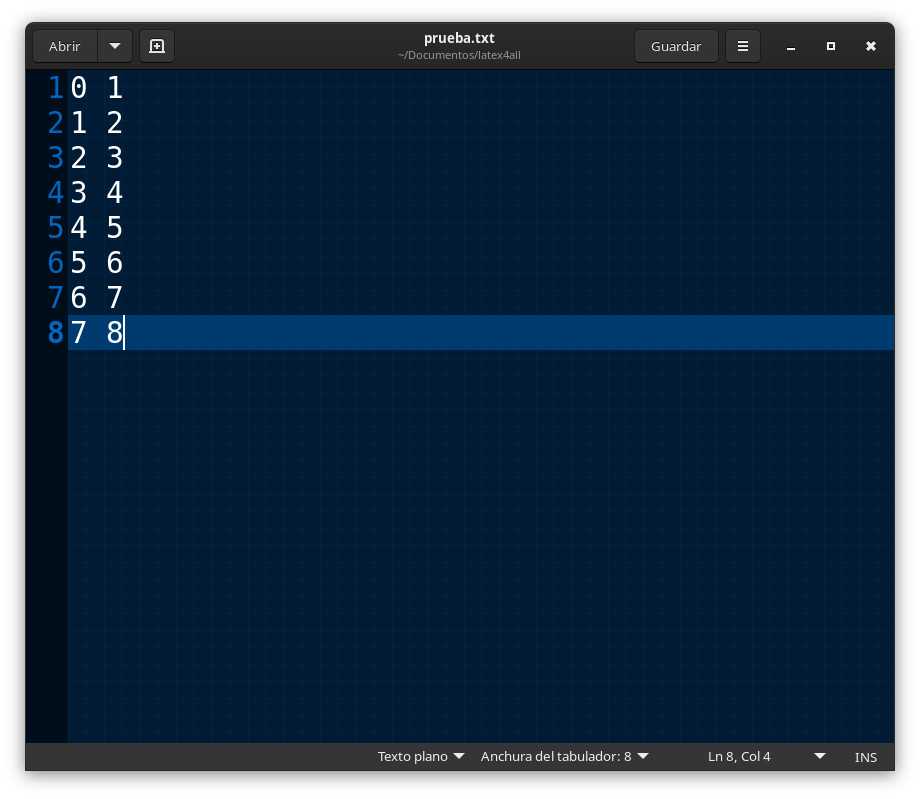
\includegraphics[width=5cm]{prueba}
		\end{minipage}\hfill\begin{minipage}{0.5\textwidth}
		\centering
		\begin{tikzpicture}[scale=0.65]
			\begin{axis}
				\addplot [color=red, mark=*, only marks] table{prueba.txt};
			\end{axis}
		\end{tikzpicture}
	\end{minipage}
	no olvides incluir en el \emph{preámbulo} la instrucción:
\begin{minted}[fontsize=\scriptsize, tabsize=3]{TeX}
\usepackage{pgfplots}
\end{minted}
		\end{mybox}
	\end{tcolorbox}
\end{document}